\section{Mato Grosso: Contexto e Dados}
\label{sec:dados}

\begingroup
\newcommand{\Hobs}{3.384}
\newcommand{\Hvalid}{2.772}
\newcommand{\Hmissing}{612}
\newcommand{\HmissingPct}{18,1}
\newcommand{\Hfixed}{95}
\newcommand{\HminFracExcl}{99,8713}
\newcommand{\HfixedObs}{2.280}
\newcommand{\Hmixed}{63}
\newcommand{\HnMin}{108}
\newcommand{\HnMax}{136}
\newcommand{\HpastShare}{91,6}
\newcommand{\HagFirst}{0,16}
\newcommand{\HagLast}{0,02}
\newcommand{\HpaFirst}{1,07}
\newcommand{\HpaLast}{0,51}
\newcommand{\HibValid}{1.760}
\newcommand{\HibComplete}{1.526}
\newcommand{\HibMin}{5}
\newcommand{\HibMax}{102}
\newcommand{\HmaxAg}{8,00}
\newcommand{\HmaxPa}{26,54}


A investigação de como os retornos econômicos esperados e o ambiente institucional condicionam a conversão da vegetação nativa requer que a expansão produtiva seja considerada em conjunto com as alternativas de uso da terra e as condições dos territórios. Para situar esse problema em Mato Grosso, são reunidas informações sobre produção agropecuária, cobertura vegetal, preços, autuações ambientais e capacidade produtiva, referentes ao período de 2001 a 2024. A análise é organizada a partir de uma grade de 141 municípios, definida pela malha do IBGE de 2023\footnote{O município de Boa Esperança do Norte, criado a partir de áreas de Sorriso e Nova Ubiratã pela Lei Estadual nº 7.264, de 29 de março de 2000, teve sua efetivação e instalação confirmadas após decisão do Supremo Tribunal Federal (STF) em outubro de 2023. Para os fins desta análise, o município não é considerado como unidade autônoma no painel de 2001-2024.}.

\subsection{Expansão agropecuária e transformação da cobertura vegetal}
\label{subsec:mt-expansao}

A trajetória agropecuária de Mato Grosso permite examinar como a ampliação da produção se relaciona com a transformação da vegetação nativa. Na perspectiva de \citeonline{Angelsen2010}, discutida na revisão da literatura, a decisão de converter depende da comparação entre os retornos apropriáveis dos usos alternativos da terra, enquanto parte dos benefícios da conservação permanece fora dessa comparação privada. A relevância da expansão produtiva para o problema deste artigo reside, portanto, nas condições em que ela envolve a abertura de novas áreas e nas atividades para as quais a vegetação é convertida.

%% Gráfico 1: Evolução das lavouras de soja e milho em Mato Grosso, 2001--2024
O Gráfico~\ref{fig:h1-lavouras} apresenta a soja na coluna da esquerda e o milho na coluna da direita. De cima para baixo, os painéis mostram a área plantada, correspondente à superfície semeada; a área colhida, correspondente à superfície em que a colheita foi efetivamente realizada; e a produção, que expressa a quantidade obtida. As duas medidas de área são apresentadas em milhões de hectares, enquanto a produção é medida em milhões de toneladas. 

Em cada ano, são somados os hectares plantados, os hectares colhidos ou as toneladas produzidas, conforme o painel. A linha azul calcula esses totais sempre para os mesmos 66 municípios produtores de soja e 121 de milho, que possuem dados em todos os anos de 2001--2024. A linha cinza tracejada inclui esses mesmos municípios e acrescenta aqueles que possuem dados naquele ano, mas não em todos os anos do período. Assim, a linha azul permite acompanhar o crescimento dentro de um grupo constante de municípios; a tracejada apresenta o total de toda a informação disponível em cada ano.

Considerando as linhas azuis, a comparação entre os painéis intermediários e inferiores permite distinguir as trajetórias das duas culturas. Na soja, à esquerda, a produção cresceu em proporção semelhante à área colhida. No milho, à direita, a produção aumentou proporcionalmente mais que a área colhida, indicando que sua expansão combinou aumento de área e maior quantidade produzida por hectare. Entre 2001 e 2024, o rendimento do milho, calculado pela divisão da produção pela área colhida, passou de 3,26 para 6,72 toneladas por hectare.

\begin{grafico}[htbp]
    \centering
    \includegraphics[width=\textwidth]{../stats/figuras/fig05_lavouras.pdf}
    \caption{Evolução das lavouras de soja e milho em Mato Grosso, 2001--2024}
    \label{fig:h1-lavouras}
    \begin{minipage}{\textwidth}\footnotesize
    Fonte: elaboração própria, com base em IBGE/PAM.

    \medskip

    \textit{A amostra fixa contém 66 municípios para soja e 121 para milho, com plantio, colheita e produção observados em todos os anos. A amostra variável contém os municípios com as três medidas disponíveis em cada ano, com cobertura municipal distinta ao longo do período. As áreas de soja e milho podem incluir cultivos sucessivos na mesma superfície física.}

    \end{minipage}
\end{grafico}
\FloatBarrier

Esse contraste ajuda a distinguir crescimento da produção e expansão sobre vegetação nativa. Além do aumento do rendimento, o cultivo sucessivo de soja e milho permite obter duas colheitas na mesma superfície, conforme discutido por \citeonline{VanWeyEtAl2013}. A ampliação da oferta pode, portanto, envolver maior aproveitamento de terras já utilizadas, o que torna necessário investigar em quais condições os incentivos produtivos resultam em novas conversões. As séries da PAM/IBGE \cite{IBGEPAM2026} permitem reconhecer mudanças de área e rendimento, mas não identificar quanto da expansão ocorreu sobre vegetação nativa.

%% Tabela 1: Escala da pecuária e das exportações em Mato Grosso -- 2001 e 2024
A distinção entre produzir mais e converter novas áreas também se aplica à pecuária. O crescimento do rebanho e do abate registrado na Tabela~\ref{tab:h1-oferta-contexto} evidencia a ampliação da atividade, mas não permite determinar quanto dessa expansão dependeu da abertura de pastagens. Em conjunto com o avanço das exportações, esses resultados descrevem a expansão da produção e de sua comercialização, dimensões que possuem expressão nos mercados. Retoma-se, nesse ponto, a assimetria discutida por \citeonline{Angelsen2010}: enquanto a exploração agropecuária pode gerar renda apropriável pelos produtores, parte dos benefícios da vegetação alcança outros agentes e não remunera diretamente quem a conserva. Por essa razão, a expansão produtiva e comercial não basta para avaliar o resultado econômico da transformação territorial para a sociedade. É necessário examinar como ela coexistiu com a conversão da vegetação e quais usos passaram a ocupar as áreas convertidas.

\input{../stats/tabelas/tab_contexto_oferta_h1}
\FloatBarrier

%% Tabela 2: Taxas agregadas de conversão da vegetação nativa para agricultura e pastagem em MT -- 2001-2024
O confronto entre expansão produtiva e conversão revela uma trajetória que qualifica a associação imediata entre crescimento agropecuário e abertura de novas áreas. No Gráfico~\ref{fig:h1-conversao}, as taxas da amostra fixa são menores em 2024 do que em 2001, tanto para agricultura quanto para pastagem, apesar da ampliação produtiva documentada anteriormente. A comparação se aproxima do resultado de \citeonline{MacedoEtAl2012}, que identificaram, na porção florestal de Mato Grosso, crescimento da produção de soja e redução do desmatamento, com expansão predominantemente em terras já abertas. A convergência está na coexistência dessas trajetórias; os diferentes períodos, recortes e amostras impedem atribuir aos dados aqui apresentados o mesmo mecanismo identificado naquele estudo. Para examinar essa distinção, são utilizadas as transições do MapBiomas \cite{MapBiomas2026}: a conversão bruta acompanha a passagem de vegetação nativa para agricultura ou pastagem, preservando a diferença entre abertura de novas áreas e reorganização de usos já agropecuários.

\begin{grafico}[htbp]
    \centering
    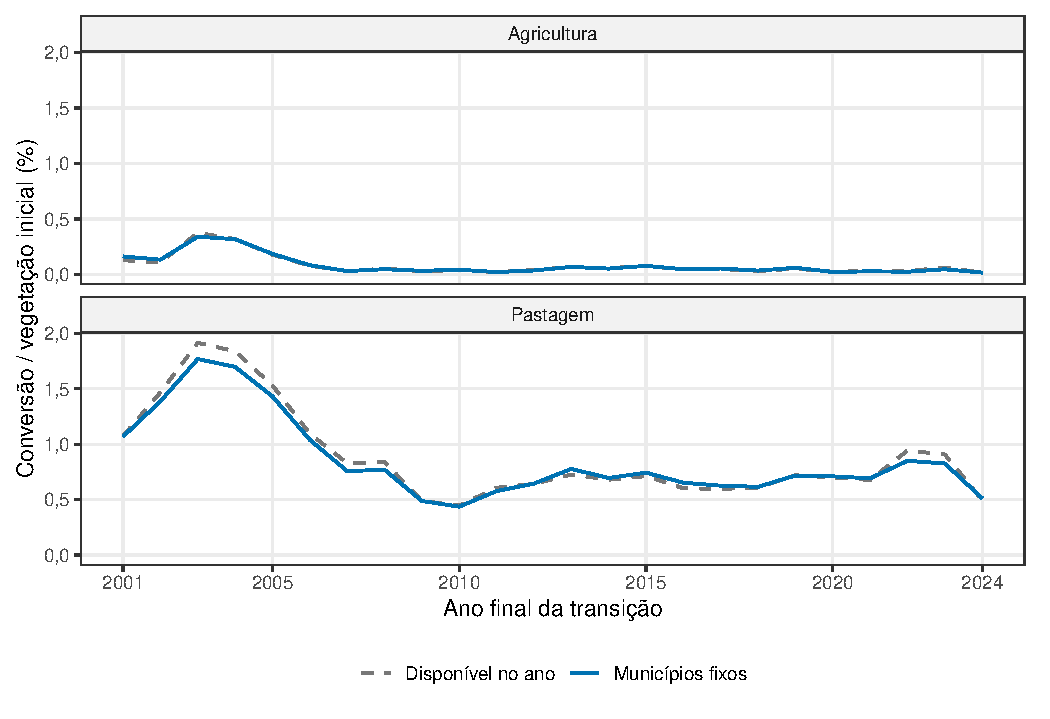
\includegraphics[width=\textwidth]{../stats/descritiva/resultados_h1/figuras/fig01_conversao.pdf}
    \caption{Taxas agregadas de conversão da vegetação nativa para agricultura e pastagem em MT -- 2001-2024}
    \label{fig:h1-conversao}
    \begin{minipage}{\textwidth}\footnotesize
    Fonte: elaboração própria com MapBiomas 10.1 e malha IBGE 2023. Cada ponto corresponde à soma da conversão dividida pela soma da vegetação nativa inicial dos mesmos municípios, multiplicada por 100. A amostra disponível varia entre \HnMin{} e \HnMax{} municípios por ano; a fixa contém \Hfixed{}. Pares incompletos não entram no numerador nem no denominador. A razão entre somas atribui maior peso aos municípios com maior estoque nativo inicial. São \Hvalid{} pares município-ano válidos e \Hmissing{} ausentes, equivalentes a \HmissingPct{}\% da grade. As taxas representam conversão bruta por destino, não perda líquida de cobertura.
    \end{minipage}
\end{grafico}

\FloatBarrier

A predominância das pastagens como destino imediato da conversão acrescenta outra dimensão a esse contraste. Embora as lavouras tenham apresentado expressiva expansão, a pastagem respondeu por \HpastShare{}\% da soma das áreas convertidas para os dois destinos nos pares município-ano válidos. Esse resultado dialoga com a persistência da conversão para pastagens descrita por \citeonline{MacedoEtAl2012} e evidencia a necessidade de considerar a pecuária na investigação dos incentivos à abertura de novas áreas. Também fundamenta o objetivo de construir medidas separadas de conversão para agricultura e pastagem: a expansão das atividades e sua participação direta nos fluxos de conversão não seguem necessariamente a mesma composição. Essa participação se restringe às observações disponíveis e não identifica eventuais relações indiretas entre a expansão das lavouras e a abertura de pastagens.

%% Ligação com H1
A combinação entre crescimento produtivo e continuidade da conversão também recupera o argumento da revisão sobre a diferença entre benefícios privados e resultados sociais. Como discutido a partir de \citeonline{Mann2012}, a avaliação econômica da conversão exige considerar os serviços associados à vegetação, além da renda obtida com seu uso produtivo. Assim, os aumentos de produção e exportação documentados não constituem um balanço dos benefícios e custos da transformação territorial. Da mesma forma, taxas menores de conversão não informam o valor dos serviços ambientais afetados pelas áreas que continuam sendo convertidas. Os dados permitem acompanhar atividades econômicas e mudanças de cobertura, mantendo em aberto a valoração de suas consequências para outros agentes e territórios.

Para a investigação de H1, a coexistência de expansão produtiva, menores taxas de conversão nos extremos do período e predominância das pastagens delimita uma questão sobre as condições da resposta aos incentivos. O crescimento da oferta pode envolver maior aproveitamento de terras já utilizadas, enquanto a abertura de novas áreas permanece como alternativa cuja atratividade depende dos retornos esperados e das restrições enfrentadas pelos agentes. O exame da hipótese requer, portanto, investigar como preços, capacidade produtiva local e ambiente institucional se relacionam com a intensidade da conversão para cada destino. A descrição fundamenta essa investigação ao mostrar que o crescimento realizado da produção e a transformação da vegetação são dimensões relacionadas, mas não intercambiáveis.

\FloatBarrier
\subsection{Preços agropecuários e incentivos à conversão}
\label{subsec:mt-precos}

As decisões de uso da terra são condicionadas pela comparação entre as rendas que podem ser obtidas com a exploração agropecuária e com a manutenção da vegetação. Na subseção sobre preços agropecuários e decisões de uso da terra, essa comparação foi situada em termos de retornos relativos, conforme o enquadramento de \citeonline{Angelsen2010}. De um lado, preços mais elevados podem ampliar a receita esperada da produção; de outro, pagamentos por serviços ambientais e receitas associadas à conservação do carbono podem tornar a manutenção da vegetação uma alternativa remunerada, conforme discutido na revisão. Essas receitas dependem de condições de acesso e implementação e não se confundem com o valor social de todos os serviços da vegetação. Como não são observadas neste conjunto de dados, a descrição dos incentivos fica concentrada nos preços dos produtos agropecuários.

Mantidos os custos e as demais condições, o acréscimo de receita por hectare decorrente de uma elevação de preço tende a ser maior onde a capacidade produtiva do uso beneficiado é mais elevada. Essa relação aproxima a investigação da abordagem de \citeonline{BermanEtAl2023}, que combinaram preços internacionais e aptidão agrícola no exame do desmatamento tropical. Entretanto, o aumento da produção também pode envolver capital, trabalho, insumos e melhor aproveitamento de áreas já utilizadas, sem expansão proporcional da superfície convertida. A resposta observada depende, portanto, das alternativas produtivas e das restrições institucionais; o preço constitui uma dimensão do incentivo, sem representar integralmente a rentabilidade esperada.

Para observar os movimentos de preços, foram utilizadas as séries da \textit{Pink Sheet} do Banco Mundial \cite{WorldBank2026}, deflacionadas mês a mês pelo CPI-U dos Estados Unidos, disponibilizado pelo BLS/FRED, para dólares de poder de compra médio de 2024 \cite{BLSCPI2026}. Soja e milho são cotados por tonelada, e carne bovina, por quilograma. No Gráfico~\ref{fig:h1-precos}, os valores são apresentados como índices com base 100 em 2000, permitindo comparar movimentos proporcionais sem equiparar unidades ou receitas por hectare. Cada média anual exige doze meses, e o preço do ano civil anterior é associado à conversão em $t$; por isso, a janela dos preços corresponde a 2000--2023.

\begin{grafico}[htbp]
    \centering
    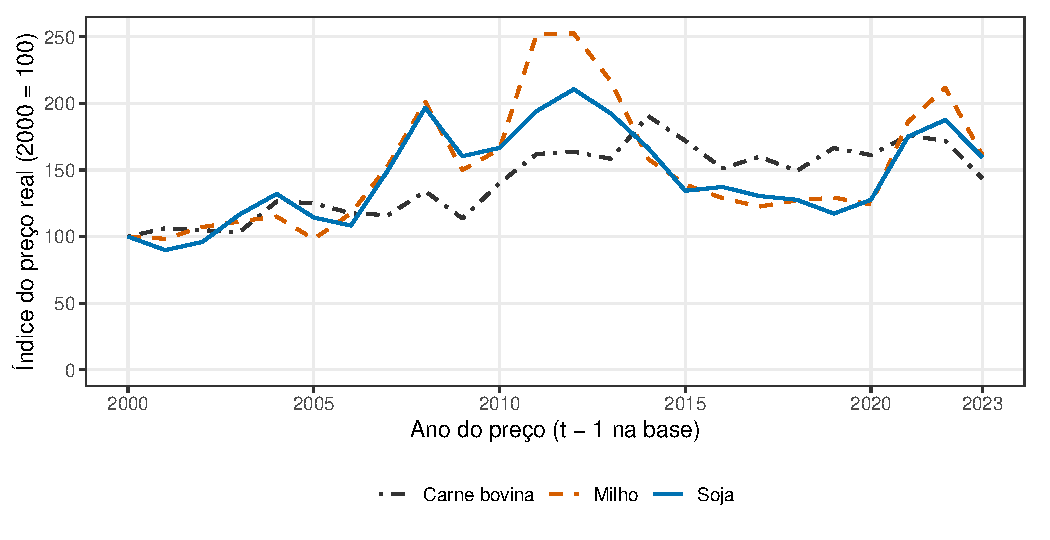
\includegraphics[width=\textwidth]{../stats/descritiva/resultados_h1/figuras/fig03_precos.pdf}
    \caption{Trajetórias dos preços reais internacionais de soja, milho e carne bovina}
    \label{fig:h1-precos}
    \begin{minipage}{\textwidth}\footnotesize
    Fonte: elaboração própria com Banco Mundial e CPI-U BLS/FRED. Índice do preço real anual de cada produto, com 2000 = 100. São 24 valores anuais distintos por produto, repetidos na grade municipal; a repetição não amplia a informação temporal. Preços de $t-1$ são associados às transições de $t$. Dólares constantes não equivalem a preços locais em reais.
    \end{minipage}
\end{grafico}

Em 2012, foram registrados índices de 210,7 para soja e 252,6 para milho, ante 163,8 para carne bovina. A valorização dos grãos não foi acompanhada proporcionalmente pela carne, cuja trajetória também diferiu nos anos seguintes. Essa diferença é relevante à luz do resultado de \citeonline{Braganca2018}: no Tapajós, aumentos do preço relativo de lavouras em relação à carne estiveram associados à substituição de pastagens por cultivos e à redução do desmatamento local. As séries apresentadas documentam movimentos relativos de preços, mas as taxas de conversão da vegetação não medem a substituição entre usos já agropecuários. Não se pode, por conseguinte, atribuir a trajetória de Mato Grosso ao mecanismo identificado naquele estudo apenas pela comparação dessas séries.

Outro contraste pode ser observado entre os extremos do período: em 2023, os preços reais dos três produtos permaneciam acima dos valores de 2000, enquanto as taxas de conversão de 2024 eram inferiores às de 2001 na amostra fixa. A coexistência dessas trajetórias não constitui rejeição de H1, cuja formulação é condicional à capacidade produtiva e ao ambiente institucional, mas evidencia a insuficiência de uma comparação direta entre tendências agregadas. As cotações internacionais não incorporam câmbio, custos locais, crédito ou expectativas individuais, e sua defasagem não assegura exogeneidade. Permanece, assim, a questão de em quais condições territoriais e institucionais os movimentos de preços se associam à conversão observada.

\FloatBarrier
\subsection{Instituições ambientais e respostas aos incentivos}
\label{subsec:mt-instituicoes}

As respostas aos incentivos econômicos também são condicionadas pelas regras de uso da terra e pelas condições de sua implementação. Conforme discutido na subseção sobre ambiente institucional e respostas aos incentivos econômicos, a existência de uma norma não assegura seu cumprimento, assim como a atuação de uma organização não resume todas as dimensões institucionais relevantes. Na Amazônia, \citeonline{AssuncaoEtAl2023} identificaram contenção do desmatamento pelo monitoramento e pela fiscalização, explorando limitações de detecção por nuvens do DETER. Para Mato Grosso, os registros de autuação permitem descrever uma dimensão dessa atuação administrativa, embora não ofereçam, isoladamente, medida equivalente de efetividade.

São considerados os autos de infração do IBAMA \cite{IBAMA2026} classificados como Flora, segundo o ano de lavratura e o município atribuído pelas coordenadas à malha de referência. A categoria abrange ocorrências além da conversão, como infrações relativas ao transporte de produtos florestais. Contabilizam-se autos, e não valores de multas aplicadas ou pagas, tampouco decisões definitivas sobre cada infração. No Gráfico~\ref{fig:h1-ibama}, a cobertura dos registros é apresentada em conjunto com a média e a mediana das contagens cuja classificação temática está completa.

\begin{grafico}[htbp]
    \centering
    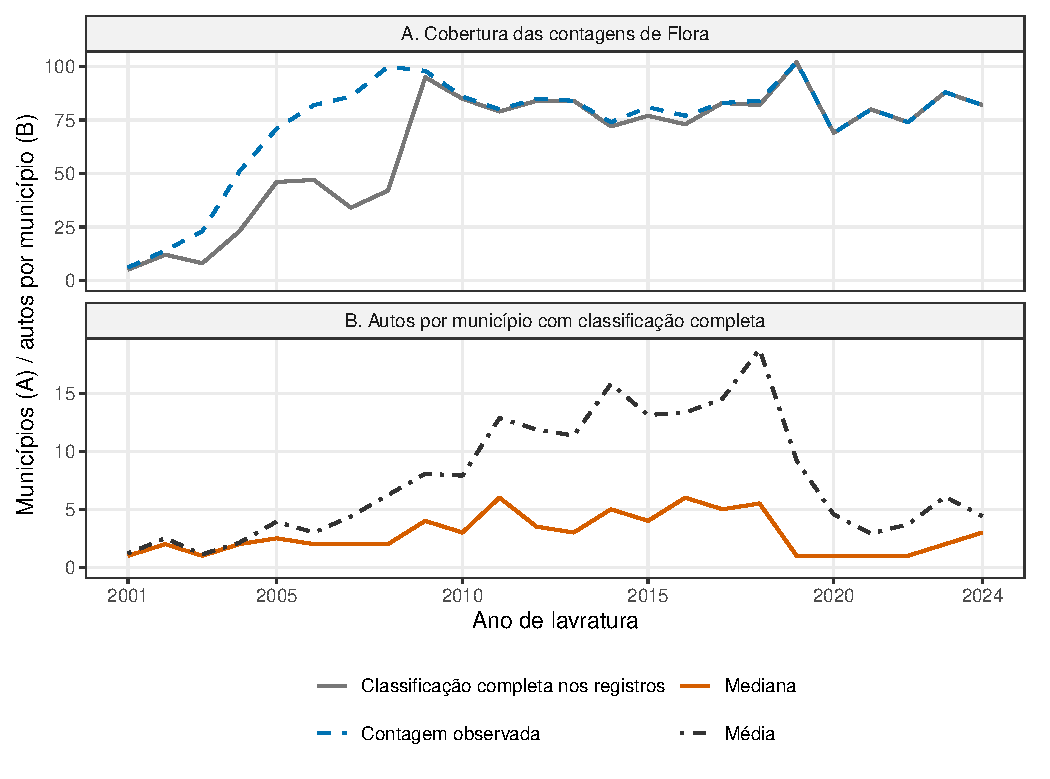
\includegraphics[width=\textwidth]{../stats/descritiva/resultados_h1/figuras/fig04_ibama.pdf}
    \caption{Cobertura e distribuição das autuações do IBAMA classificadas como Flora}
    \label{fig:h1-ibama}
    \begin{minipage}{\textwidth}\footnotesize
    Fonte: elaboração própria com registros do IBAMA e malha IBGE 2023. Painel A: municípios com contagem observada e com classificação temática completa nos registros. Painel B: média e mediana entre os municípios do segundo conjunto, de composição variável. O período contém \HibValid{} contagens observadas e \HibComplete{} com classificação completa. Ausência não é zero; classificação completa não certifica a completude da fonte ou da fiscalização. Os painéis possuem unidades e escalas distintas.
    \end{minipage}
\end{grafico}

A cobertura variou entre \HibMin{} e \HibMax{} municípios com classificação completa por ano, limitando a comparação direta das contagens. Em 2018, foram observadas média de 18,77 autos e mediana de 5,5; em 2024, esses valores corresponderam a 4,41 e 3. Nos dois anos havia 82 municípios com classificação completa, mas o mesmo tamanho não assegura a mesma composição. A distância entre média e mediana indica a influência das contagens mais elevadas em parte dos municípios. Os zeros, por sua vez, representam ausência de autos de Flora entre os registros integralmente classificados daquele município-ano, sem comprovar ausência de infrações ou de atuação fiscalizatória.

A redução da média entre esses anos admite interpretações distintas. As contagens podem variar com a incidência de infrações, o esforço de fiscalização e as condições de registro e localização, processos que podem ocorrer simultaneamente. Não se pode concluir, apenas por sua redução, que a fiscalização tenha se tornado mais eficaz ou menos presente; pela mesma razão, uma associação positiva entre autuações e conversão não demonstraria ineficácia institucional. As condições de identificação do estudo de \citeonline{AssuncaoEtAl2023} não são reproduzidas por essa descrição. Para o exame de H1, deverá ser justificado em que sentido a medida representa o condicionamento institucional, considerando que normas informais, cumprimento das sanções e atuação de outras organizações permanecem fora desse indicador.

Além da fiscalização pública, as relações comerciais podem incorporar condições ambientais ao acesso aos mercados, como discutido na revisão a propósito da Moratória da Soja e de outros instrumentos de conservação. A trajetória das exportações permite situar a escala dessas relações econômicas em Mato Grosso. No Gráfico~\ref{fig:h1-exportacoes}, são apresentados o valor FOB e o peso líquido das exportações registradas por domicílio fiscal, separadamente para soja, milho e carne bovina. O peso líquido registrado em 2024 correspondeu a 22,79 milhões de toneladas de soja, 25,28 milhões de toneladas de milho e 0,51 milhão de toneladas de carne bovina. A expansão em relação ao início do período ocorreu com oscilações: entre 2023 e 2024, valor e peso recuaram para os grãos, enquanto aumentaram para a carne bovina.

\begin{grafico}[htbp]
    \centering
    \includegraphics[width=\textwidth]{../stats/figuras/fig09_exportacoes.pdf}
    \caption{Valor e peso líquido das exportações registradas por domicílio fiscal em Mato Grosso}
    \label{fig:h1-exportacoes}
    \begin{minipage}{\textwidth}\footnotesize
    Fonte: elaboração própria com MDIC/SECEX, Comex Stat. SH4 1201 (soja), 1005 (milho) e 0201+0202 (carne bovina), 2001--2024. Valores FOB em bilhões de dólares correntes e peso líquido em milhões de toneladas, com escalas próprias em cada painel. Somam-se os registros observados, com cobertura municipal variável; ausências não são imputadas como zero. O domicílio fiscal não identifica a origem municipal da produção nem a conformidade ambiental das operações.
    \end{minipage}
\end{grafico}

O crescimento do comércio externo contextualiza a relevância das regras que podem incidir sobre as cadeias produtivas, mas não permite avaliar sua aplicação ou seus efeitos. Os registros não identificam quais operações estiveram submetidas a compromissos de conservação, nem permitem relacionar diretamente o município exportador à área de produção ou à vegetação convertida. Portanto, a evolução das exportações não deve ser tomada como evidência de êxito ou fracasso dos instrumentos ambientais. Em conjunto, os dados de comércio e autuação situam a atividade econômica e uma dimensão da atuação estatal, mantendo em aberto como as condições institucionais modificam a resposta da conversão aos incentivos de mercado.

\FloatBarrier
\subsection{Heterogeneidade econômica e ambiental de Mato Grosso}
\label{subsec:mt-heterogeneidade}

A distribuição territorial das atividades e da vegetação qualifica as tendências agregadas de Mato Grosso. Na subseção correspondente da revisão, a diversidade de trajetórias foi discutida a partir, entre outras evidências, dos mapas de \citeonline{SimoesEtAl2020}, referentes a 2001--2017. A Figura~\ref{fig:h1-uso-solo} acrescenta uma comparação cartográfica entre 2001 e 2024, elaborada com camadas do MapBiomas e classes agregadas para esta representação. Observa-se maior presença da classe denominada ``Soja e Milho'' na porção central e em áreas a leste, enquanto a cobertura florestal permanece mais concentrada ao norte. Essa distribuição situa as atividades em contextos ambientais distintos, sem supor que todos os municípios de um mesmo bioma compartilhem a mesma trajetória.

\begin{figure}[htbp]
    \centering
    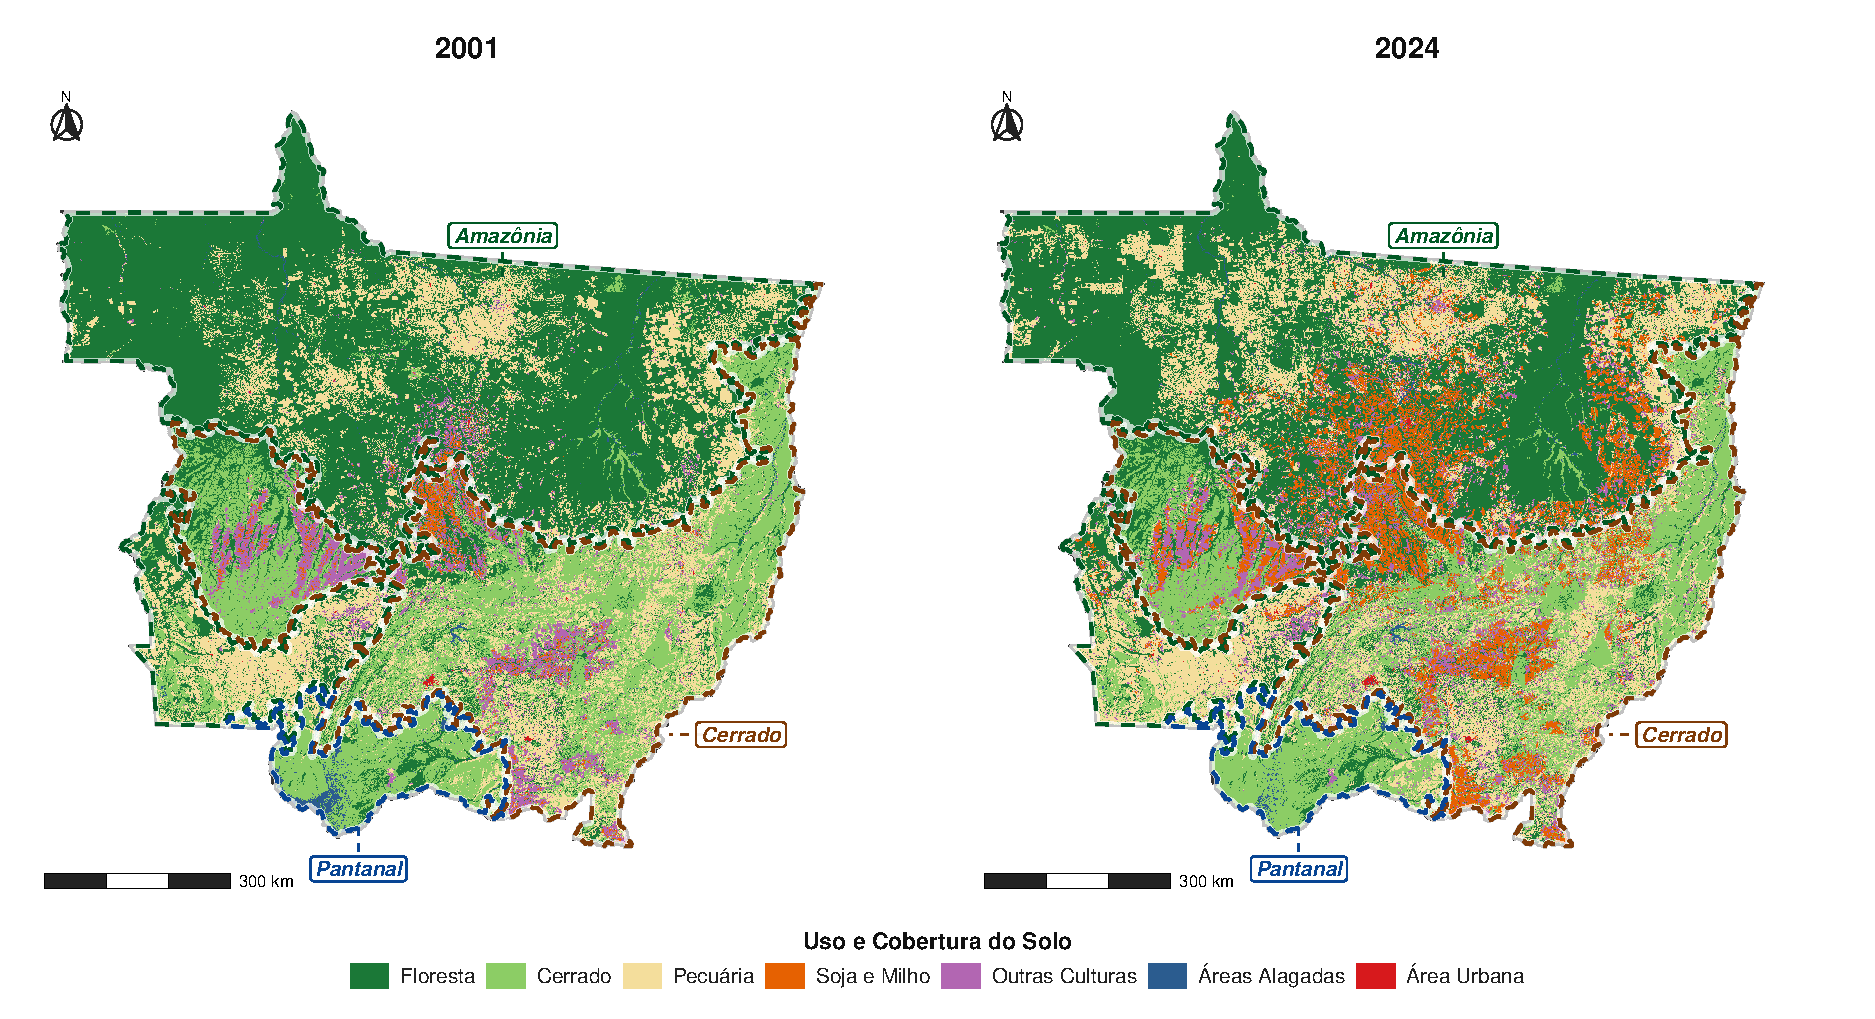
\includegraphics[width=\textwidth]{../stats/descritiva/simoes2020/fernando/outputs/fig6_uso_solo_mt_2001_2024.pdf}
    \caption{Distribuição espacial de classes agregadas de uso e cobertura do solo em Mato Grosso, 2001 e 2024}
    \label{fig:h1-uso-solo}
    \begin{minipage}{\textwidth}\footnotesize
    Fonte: elaboração própria com camadas do MapBiomas e limites do IBGE, em SIRGAS 2000; escala de extração dos rasters de 500 m. Trata-se de representação derivada, não dos mapas originais de Simões et al. (2020). Na legenda, ``Pecuária'' representa pastagens; ``Cerrado'' reúne formações savânicas, campestres e outras formações nativas, não o limite do bioma; ``Áreas Alagadas'' corresponde a corpos d'água. ``Outras Culturas'' também inclui vegetação secundária e classes residuais, não podendo ser interpretada exclusivamente como área cultivada. As classes cartográficas não substituem as medidas anuais de conversão bruta.
    \end{minipage}
\end{figure}

\FloatBarrier
A comparação entre os dois mapas descreve a configuração da cobertura em cada data, sem identificar a sequência anual de transições ou separar expansão sobre vegetação de substituições entre usos já agropecuários. Sua legenda também exige cautela: a classe ``Outras Culturas'' reúne coberturas de naturezas distintas, inclusive vegetação secundária. Por isso, a figura é utilizada para contextualizar a distribuição espacial, e não para calcular a perda total de vegetação nativa ou a expansão líquida das lavouras. A investigação municipal apresentada a seguir se apoia nas medidas de conversão já definidas, com critérios próprios de cobertura e agregação.

Para essa comparação, os municípios foram agrupados pelo bioma com a maior fração de sua área, obtida pela interseção da malha municipal de 2023 com os biomas do IBGE de 2019. Foram preservadas as frações originais, e \Hmixed{} municípios apresentam mais de um bioma. Conforme a Tabela~\ref{tab:h1-cobertura}, a conversão foi observada em 71,6\% dos pares potenciais no grupo de predominância amazônica, 96,4\% no Cerrado e 56,2\% no Pantanal. Dos quatro municípios de predominância pantaneira, somente um possui informação em todos os anos. A amostra fixa reduz alterações de composição ao longo do tempo, mas não torna os grupos igualmente informativos nem resolve a compatibilidade histórica de todas as séries administrativas.

\begin{table}[htbp]
\centering
\small
\caption{Cobertura da conversão por predominância territorial, 2001--2024}\label{tab:h1-cobertura}
\begin{tabular}{lrrrrr}
\hline
Grupo & Municípios & Mistos & Pares válidos & \% da grade & Fixos \\
\hline
Amazônia & 76 & 35 & 1.306 & 71,6 & 39 \\
Cerrado & 61 & 24 & 1.412 & 96,4 & 55 \\
Pantanal & 4 & 4 & 54 & 56,2 & 1 \\
\hline
\end{tabular}
\par\smallskip\begin{minipage}{\textwidth}\footnotesize
Fonte: elaboração própria com MapBiomas 10.1 e IBGE.
\end{minipage}
\end{table}

\FloatBarrier

As diferenças dentro e entre esses grupos podem ser observadas no Gráfico~\ref{fig:h1-distribuicao}. Cada ponto representa a média das 24 taxas anuais de um município da amostra fixa, atribuindo peso igual aos anos, diferentemente da razão entre somas do Gráfico~\ref{fig:h1-conversao}. Para pastagem, a mediana dessas médias foi de 1,42\% nos 39 municípios de predominância amazônica e de 0,73\% nos 55 de predominância Cerrado. Em ambos os grupos, há dispersão e municípios com valores superiores aos resumos centrais. Para agricultura, as taxas médias são menores, mas também heterogêneas. O único município pantaneiro não permite caracterizar uma distribuição ou estabelecer uma comparação representativa com os demais grupos.

\begin{grafico}[htbp]
    \centering
    \includegraphics[width=\textwidth]{../stats/figuras/fig02_distribuicao.pdf}
    \caption{Heterogeneidade das taxas médias municipais de conversão, 2001--2024}
    \label{fig:h1-distribuicao}
    \begin{minipage}{\textwidth}\footnotesize
    Fonte: elaboração própria com MapBiomas 10.1 e IBGE. Cada ponto é a média aritmética das 24 taxas anuais de um município da amostra fixa. O deslocamento horizontal aleatório apenas separa os pontos; a altura preserva a taxa observada. Grupos definidos pelo bioma predominante na área municipal, sem rateio da conversão pelas frações de bioma. Todos os municípios fixos são mostrados; o grupo pantaneiro contém uma única observação municipal.
    \end{minipage}
\end{grafico}

Essas diferenças complementam a caracterização territorial da literatura ao mostrar que a heterogeneidade não se restringe à comparação entre biomas. Municípios de um mesmo grupo podem diferir em vegetação disponível, estrutura produtiva, acesso a mercados e condições institucionais. Além disso, a predominância territorial não localiza cada conversão no interior de um bioma: os fluxos municipais não foram repartidos pelas frações de área, pois essa operação lhes atribuiria uma localização não informada pelos agregados. As diferenças descritivas não isolam, assim, um efeito do bioma sobre a conversão.

A capacidade produtiva acrescenta outra dimensão à comparação. Na Tabela~\ref{tab:h1-capacidade}, são apresentados os rendimentos potenciais do GAEZ v4 \cite{FAOGAEZ2021}, no cenário de alto insumo e sequeiro. Para soja, a mediana municipal foi de 2.701 kg de matéria seca por hectare no grupo amazônico e de 3.261 no Cerrado; para milho, de 3.002 e 3.320, respectivamente. Os intervalos interquartis registram diferenças também no interior dos grupos. São considerados os 141 municípios, uma única vez cada, e não apenas os 95 da amostra fixa de conversão. Dessa forma, as posições relativas dos grupos nas duas distribuições não constituem estimativa da relação entre capacidade produtiva e conversão.

\begin{table}[htbp]
\centering
\small
\caption{Rendimento potencial municipal no cenário de alto insumo e sequeiro}\label{tab:h1-capacidade}
\begin{tabular}{llrrr}
\hline
Cultura & Predominância & Municípios & Mediana & P25--P75 \\
\hline
Milho & Amazônia & 76 & 3.002 & 2.862--3.264 \\
Milho & Cerrado & 61 & 3.320 & 2.797--3.572 \\
Milho & Pantanal & 4 & 6.790 & 6.321--6.933 \\
Soja & Amazônia & 76 & 2.701 & 2.557--2.852 \\
Soja & Cerrado & 61 & 3.261 & 2.817--3.390 \\
Soja & Pantanal & 4 & 3.421 & 3.386--3.457 \\
\hline
\end{tabular}
\par\smallskip\begin{minipage}{\textwidth}\footnotesize
Fonte: elaboração própria com FAO/IIASA, GAEZ v4, clima 1961--1990 e terras de 2010; agregação municipal na malha IBGE 2023. Unidade: kg de matéria seca por hectare. Cada município entra uma vez, com peso igual. P25--P75 delimita a metade central da distribuição. O cenário não representa o rendimento realizado nem garante capacidade predeterminada em relação a todo o painel.
\end{minipage}
\end{table}

\FloatBarrier

A distinção entre rendimento potencial e realizado, desenvolvida na revisão, é relevante para a interpretação dessa medida. O rendimento da PAM é obtido nas áreas colhidas e responde ao manejo, aos insumos e à seleção das parcelas cultivadas. No GAEZ, os pixels válidos foram agregados por município com ponderação pelo cosseno da latitude, aproximando diferenças de área, enquanto os resumos entre municípios lhes atribuem peso igual. A referência combina clima de 1961--1990 e informações de terras de 2010, não assegurando predeterminação integral em relação ao painel. Matéria seca e unidades comerciais também precisam ser compatibilizadas antes de uma combinação com preços, e não há medida validada de capacidade pecuária neste conjunto. A heterogeneidade observada situa, portanto, a pertinência de investigar respostas diferenciadas, mantendo a escolha das medidas predeterminadas e o suporte das comparações como questões da estratégia econométrica.

\subsection{Síntese e articulação com a estratégia econométrica}
\label{subsec:mt-sintese}

A descrição de Mato Grosso documenta expansão agropecuária e comercial, taxas agregadas de conversão menores nos extremos do período e predominância da pastagem nos fluxos observados. Ao mesmo tempo, foram identificados movimentos distintos de preços, distribuição territorial desigual das atividades, dispersão das taxas municipais e diferenças de capacidade produtiva, enquanto os registros de autuação apresentam cobertura variável e interpretação institucional limitada. Esses resultados delimitam o problema de como os retornos econômicos esperados e o ambiente institucional condicionam a conversão, em consonância com os objetivos de construir medidas brutas por destino e examinar suas relações com preços, capacidade produtiva e condições institucionais, considerando atividades e biomas. É nesse sentido que se articula H1: \emph{Elevações nos retornos econômicos esperados dos usos agropecuários aumentam a taxa de conversão da vegetação nativa, sendo essa resposta, \textit{ceteris paribus}, amplificada pela capacidade produtiva local da terra e modulada pela efetividade do ambiente institucional.} A descrição permite reconhecer a coexistência e a heterogeneidade dessas dimensões, mas não confirma ou rejeita a hipótese; permanece em aberto a intensidade com que os incentivos se associam à conversão sob diferentes condições locais.

O aprofundamento dessa questão requer que a variação dos incentivos seja distinguida de tendências comuns, diferenças persistentes entre territórios, seleção amostral e respostas da fiscalização às próprias infrações. Na Seção~\ref{sec:estrategia}, deverá ser desenvolvido o desenho geral anunciado na introdução, com dados em painel, ordenação temporal entre preços e conversão, interações com capacidade produtiva e condições institucionais, efeitos fixos territoriais e temporais e controles compatíveis com a investigação. A definição das especificações dependerá da justificativa das medidas, da amostra e do suporte de cada comparação, especialmente diante da cobertura restrita do Pantanal e das limitações temporais do GAEZ. Esses procedimentos não asseguram, por si sós, identificação causal; quando suas condições não puderem ser sustentadas, os resultados deverão ser interpretados como associações condicionais. A evidência descritiva estabelece, assim, os objetos e os limites a partir dos quais poderá ser aprofundada a investigação econométrica de H1.

\endgroup
